% --- Books ---
% - https://www.amazon.de/Docker-Software-entwickeln-deployen-Containern/dp/386490384X/ref=sr_1_1?ie=UTF8&qid=1483784437&sr=8-1&keywords=docker
% - https://www.amazon.com/Docker-Action-Jeff-Nickoloff/dp/1633430235/ref=sr_1_1?ie=UTF8&qid=1483784469&sr=8-1&keywords=docker
% - https://www.amazon.com/Docker-Practice-Ian-Miell/dp/1617292729/ref=sr_1_10?ie=UTF8&qid=1483784469&sr=8-10&keywords=docker
% - https://www.amazon.com/Developing-Docker-Jaroslaw-Krochmalski-ebook/dp/B01GEJKJ6A/ref=sr_1_33?ie=UTF8&qid=1483784510&sr=8-33&keywords=docker

\chapter{Docker}
\label{cha:docker}
Wie in \cref{sec:vollvirtualisierung} beschrieben, ermöglicht die Virtualisierung von IT-Systemen Abstraktion von der Hardware.
Ressourcen lassen sich effizienter ausnützen, die Systeme werden jedoch nur suboptimal ausgenützt, da das gesamte Betriebssystem virtualisiert wird.
Dies führt zu langen Startzeiten und einem hohen Speicherverbrauch.

Containervirtualisierung (siehe \cref{sec:containervirtualisierung}) löst diese Probleme durch die Wiederverwendung des Kernels.
Dadurch entsteht die Möglichkeit Anwendungen mitsamt der benötigten Systemressourcen zu verpacken und die Abhängigkeiten für den Betrieb zu reduzieren.
Für einen Container wird lediglich die Laufzeitumgebung benötigt, ist diese installiert, ist garantiert, dass der Container funktioniert.
Docker\footnote{\url{https://www.docker.com/}} wird in 94\% (Stand Juni 2016) der Unternehmen eingesetzt, die auf Containervirtualisierung setzen \autocite{ContainerAdoption}.

\section{Geschichte}
\label{sec:docker-history}
Der Blogeintrag \autocite{redhat-container-history:online} schildert die Geschichte der Containervirtualisierung.

Im Jahr 2001 ermöglicht Jacques Gélinas mithilfe eines gepatchten Kernels zum ersten Mal das Ausführen mehrerer Linux-Server auf einem einzelnen Rechner, ohne auf Vollvirtualisierung zurückzugreifen.

2006 folgt die Aufnahme von cgroups in den Linux-Kernel, worauf 2008 die Implementierung der namespaces folgen.
Ebenfalls 2008 beginnt IBM mit der Entwicklung von LXC, wobei auf cgroups und namespaces aufgesetzt wird.
% http://searchservervirtualization.techtarget.com/feature/A-brief-history-of-Docker-Containers-overnight-success
% http://blog.aquasec.com/a-brief-history-of-containers-from-1970s-chroot-to-docker-2016

2013 wird Docker als Open-Source-Projekt der Platform-as-a-Service-Umgebung dotCloud vorgestellt.
Docker führt nichts wesentlich Neues ein, sondern bietet lediglich für die bestehenden Technologien wie LXC eine sehr einfach zu verwendende Benutzerschnittstelle, die Container für eine breite Benutzergruppe zugänglich macht.

2014 erscheint Docker in der Version 1.0, nachdem mit Version 0.9 LXC als Containerumgebung durch \emph{libcontainer\footnote{\url{https://github.com/opencontainers/runc/tree/master/libcontainer}}} ersetzt wird.
libcontainer ist eine Eigenentwicklung von Docker, die in der Programmiersprache Go geschrieben ist und die Verwaltung und Ausführung von Containern ermöglicht.

2015 tritt Docker der Open Container Initiative bei, wodurch die Quelltexte und Entwicklungen dem unter der Linux Foundation stehenden Projekt hinzugefügt werden.
Dieser Schritt verstummt Kritiker, die eine Monopolstellung von Docker befürchtet haben.
Seit 2015 werden hauptsächlich Fehlerbehebungen und Verbesserungen an Docker selbst durchgeführt, sowie das Docker-Ökosystem durch zahlreiche Werkzeuge erweitert (siehe \cref{sec:docker-products}).

Die in diesem Kapitel gezeigten Beispiele und verwendeten Funktionen basieren auf der Docker-Version 1.13 vom 19. Jänner 2017.
\section{Funktionsweise}
\label{sec:docker-basics}
Die Funktionsweise von Docker wird in ZITAT beschrieben und im folgenden Abschnitt zusammengefasst.
\subsection{Komponenten am Beispiel der Bash}
\label{sec:components-bash}
Ein Basiswissen über die folgenden Komponenten des Docker-Systems ist für die Verwendung von Docker unerlässlich.
\begin{description}
    \item [daemon] Im Hintergrund von Docker läuft der Server-Prozess, genannt \texttt{daemon}, der sich um das Anlegen und Verwalten von \texttt{images}, \texttt{containern}, \texttt{networks} und \texttt{data volumes} kümmert.
    Er läuft auf dem Host-System und nimmt Kommandos der \texttt{clients} über eine REST-Schnittstelle entgegen.
    \item [client] Der \texttt{client} ist die Benutzeroberfläche von Docker, die in Form einer Kommandozeilenapplikation zur Verfügung gestellt wird.
    Er nimmt Kommandos und Konfigurationen entgegen und sendet diese an einen Konfigurierten \texttt{daemon}.
    \item [engine] Als \texttt{engine} wird die Kombination aus \texttt{daemon} und \texttt{client} bezeichnet, die den Kern von Docker bilden.
    \item [image] Ein \texttt{image} ist eine Vorlage für das Erstellen eines \texttt{containers}. \texttt{Images} können erweitert und dadurch wiederverwendet werden und bilden die Basis zum Erstellen eines \texttt{containers}. Es wird idealerweise über ein \cref{sec:dockerfiles} erstellt.
    \item [container] \texttt{Container} sind jene Teile, die von Docker ausgeführt werden. Er ist eine ausführbare Instanz eines \texttt{images}. \texttt{Container} werden vom \texttt{daemon} gestartet, gestoppt, verschoben oder gelöscht, der die Anweisungen vom \texttt{client} enthält. Zusätzlich können \texttt{container} zur Inter-Container-Kommunikation Netzwerken zugewiesen werden, oder zur Datenpersistierung mit Speicherbereichen versorgt werden.
    \item [registry] \texttt{Registrys} dienen der Verteilung von \texttt{images}. Sie stellen eine Bibliothek dieser dar. Sie können entweder privat oder öffentlich zugänglich sein (siehe \cref{sec:docker-hub}).
    \item [service] Ein \texttt{service} ist eine Sammlung von Docker-Containern, welche durch einen Schwarmmanger (siehe \cref{sec:docker-swarm}) verwaltet werden und die Basis für Multi-Container-Anwendungen (siehe \cref{sec:docker-multi-container-anwendungen}) darstellen. Seit Docker 1.12 werden \texttt{services} in vollem Ausmaß unterstützt.
\end{description}
In \cref{lst:docker-run-basics} wird ein neuer Container auf Basis des Ubuntu-Images gestartet, in dem die Bash ausgeführt wird.
\begin{lstlisting}[caption=Ubuntu-Bash in Docker, language=bash, label=lst:docker-run-basics]
    $ docker run -i -t ubuntu /bin/bash
\end{lstlisting}
Dabei erledigt die Docker-Engine folgende Schritte:
\begin{enumerate}
    \item Das \texttt{ubuntu}-Docker-Image wird von der Docker-Registry heruntergeladen, falls dieses lokal noch nicht existiert.
    \item Ein neuer Container wird auf Basis des Images erstellt und mit einem zufälligen Namen versehen.
    \item Ein schreibfähiges Dateisystem wird zu dem eben erstellten Container hinzugefügt.
    \item Für den Container wird eine Netzwerkverbindung geschaffen, die eine Kommunikation mit dem Host ermöglicht. Standardmäßig wird die \texttt{bridged}-Schnittstelle verwendet.
    \item Der Container erhält eine IP-Adresse.
    \item Das angegebene Programm wird ausgeführt. In diesem Fall ist das \lstinline{/bin/bash}.
    \item Die Parameter \lstinline{-t} und \lstinline{-i} führen dazu, dass die Standardeingabe und Standardausgabe verbunden werden und der Container in einen interaktiven Modus geschaltet wird. Der Benutzer befindet sich nun in der Bash in Ubuntu in Docker.
\end{enumerate}
In \cref{fig:docker-architektur} ist dieser Ablauf grafisch dargestellt.
\begin{figure}[htbp]
    \centering
    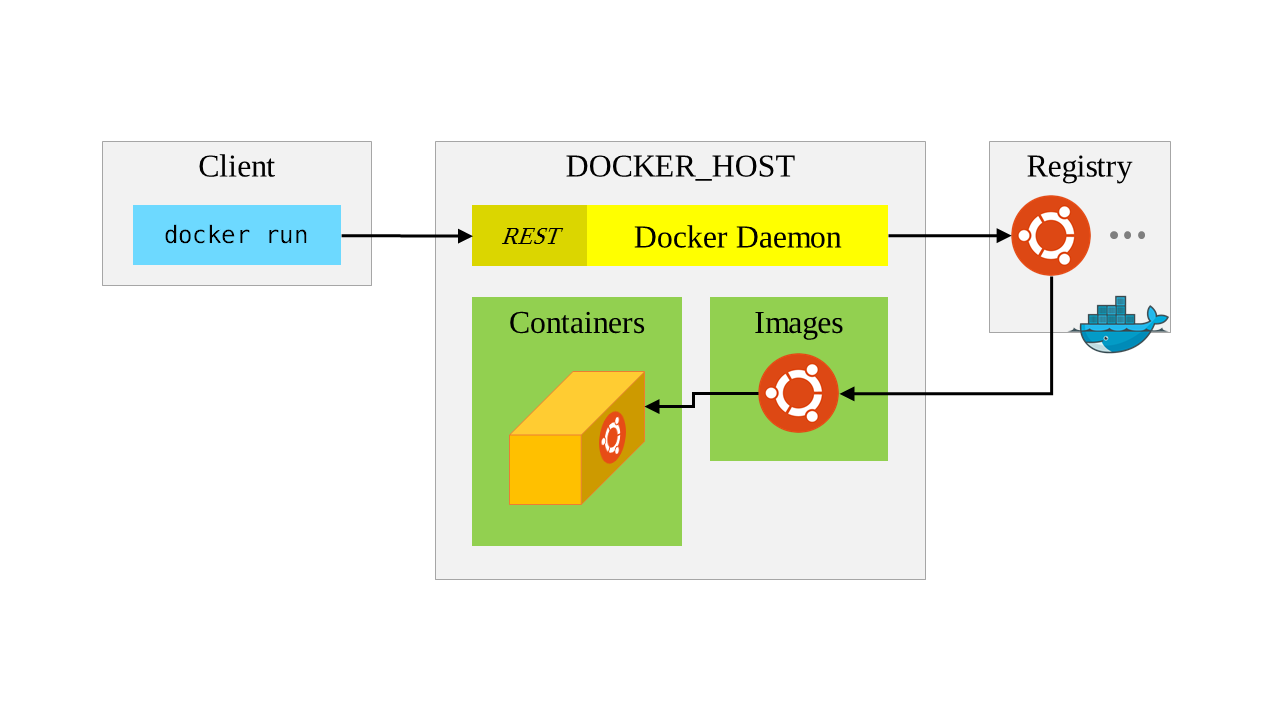
\includegraphics[width=0.9\linewidth,clip]{images/docker-architecture}
    \caption{Docker-Architektur}
\label{fig:docker-architektur}
\end{figure}
\subsection{Dateisystem}
\label{sec:filesystem}
\begin{figure}[htbp]
    \centering
    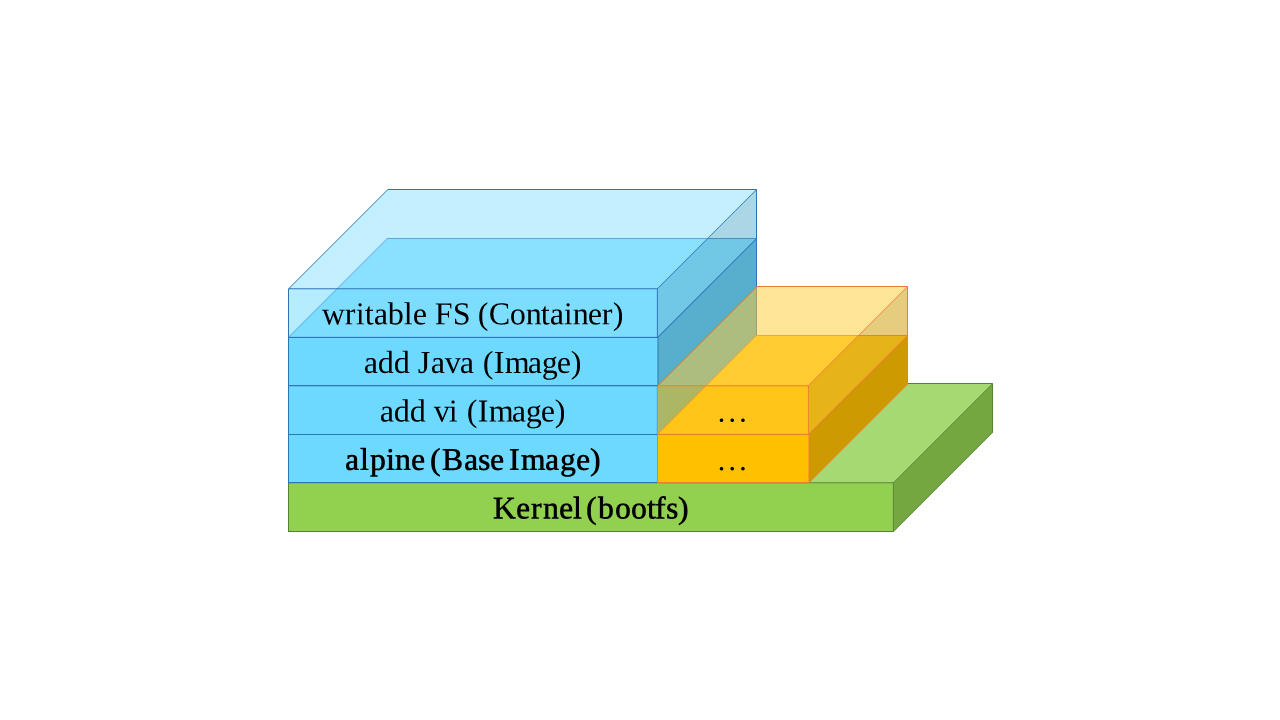
\includegraphics[width=0.7\linewidth,clip,trim=130 130 130 110]{images/docker-filesystem}
    \caption{Docker-Dateisystem}
\label{fig:docker-dateisystem}
\end{figure}
Networking
\section{Plattformen}
\label{sec:docker-platforms}
\subsection{Docker Toolbox}
\label{sec:docker-toolbox}
\subsection{Docker for Windows}
\label{sec:docker-windows}
\subsection{Docker for Mac}
\label{sec:docker-mac}
\subsection{Docker for AWS/Azure}
\label{sec:docker-cloud}

% - die Geschichte von Docker
% - Docker Aufbau, LXC, usw...
% - https://youtu.be/9CuClvKMt04?t=1m12s
% - Plattformunterschiede, Docker-Toolbox, Native-Docker, mein Docker Setup
% - Docker Windows 10
%   - http://stackoverflow.com/questions/41338203/import-module-posh-docker-is-not-working
%   - https://github.com/samneirinck/posh-docker
%   - http://stackoverflow.com/questions/39133098/how-to-mount-a-windowss-folder-in-docker-using-powershell-or-cmd
%   - http://superuser.com/questions/1051520/docker-windows-container-how-to-mount-a-host-folder-as-data-volume-on-windows
%   - https://github.com/docker/for-win/issues/328
%   - https://rominirani.com/docker-on-windows-mounting-host-directories-d96f3f056a2c
% - Clean up: https://lebkowski.name/docker-volumes/
\section{Produkte}
\label{sec:docker-products}
\subsection{Docker Hub}
\label{sec:docker-hub}
\subsection{Docker Machine}
\label{sec:docker-machine}
\subsection{Docker Compose}
\label{sec:docker-compose}
\subsection{Docker Swarm}
\label{sec:docker-swarm}


% - swarm
% - compose
% - stack
% - cli
% - machine
% - ...
% - http://portainer.io/portainer-comparison.html
% - https://media-glass.es/portainer-the-ui-for-docker-d067f6335f23#.yuokl7w7n
\section{Dockerfiles}
\label{sec:dockerfiles}
\subsubsection{CMD vs. ENTRYPOINT}

% - Layers
% - ...
% - http://bitjudo.com/blog/2014/03/13/building-efficient-dockerfiles-node-dot-js/
% - Example: https://nodejs.org/en/docs/guides/nodejs-docker-webapp/ (http://jdlm.info/articles/2016/03/06/lessons-building-node-app-docker.html)
% - https://www.brandpending.com/2016/06/14/building-nodejs-with-npm-dependencies-into-a-docker-container-without-using-a-dockerfile/ ???
% - Faster Builds: http://thenewstack.io/understanding-the-docker-cache-for-faster-builds/
% - Building good Images
% - https://blog.replicated.com/2016/02/05/refactoring-a-dockerfile-for-image-size/
% - https://nickjanetakis.com/blog/alpine-based-docker-images-make-a-difference-in-real-world-apps
% - http://blog.xebia.com/create-the-smallest-possible-docker-container/

% - ENTRYPOINT vs. CMD
% - https://www.ctl.io/developers/blog/post/dockerfile-entrypoint-vs-cmd/
% - http://goinbigdata.com/docker-run-vs-cmd-vs-entrypoint/
% - http://www.projectatomic.io/docs/docker-image-author-guidance/
\section{Multi-Container-Anwendungen} % - Namen überdenken!!!
\label{sec:docker-multi-container-anwendungen}
% - fig vs. docker-compose
% - Bash-Skripte vs. docker-compose
% - bei größeren Systemen auf Kapitel 1 (Orchestration) verweisen
% - https://ypereirareis.github.io/blog/2015/05/04/docker-with-shell-script-or-makefile/
% - http://codereview.stackexchange.com/questions/137877/shell-script-wrapper-for-docker-build-and-run
% - https://github.com/JonathonReinhart/scuba -> Simple Container-Utilizing Build Apparatus
% - https://blog.codeship.com/cross-platform-docker-development-environment/
% - stack
%  - https://docs.docker.com/docker-cloud/apps/stacks/
%  - https://blog.nimbleci.com/2016/09/14/docker-stacks-and-why-we-need-them/
%  - https://blog.couchbase.com/2016/july/docker-services-stack-distributed-application-bundle
\section{Häufige Docker-Kommandos und deren Verwendung}
\label{docker-kommandos}
% - http://jimhoskins.com/2013/07/27/remove-untagged-docker-images.html
% - Scripting
% - https://rominirani.com/docker-management-commands-e89a23c55908#.wlq1ixs5i
